\section{Conventions principales}

\textcolor{red}{Préciser la convention ISO des faces ? (page 29 Ricordeau)}

Toutes les images suivantes sont issues des animations flashs données sur moodle.

\subsection{Solides de révolution}
Losque l'on dessine une \textbf{forme de révolution}, il faut indiquer l'axe de révolution par un \textbf{trait mixte}

\begin{figure}[H]
    \centering
    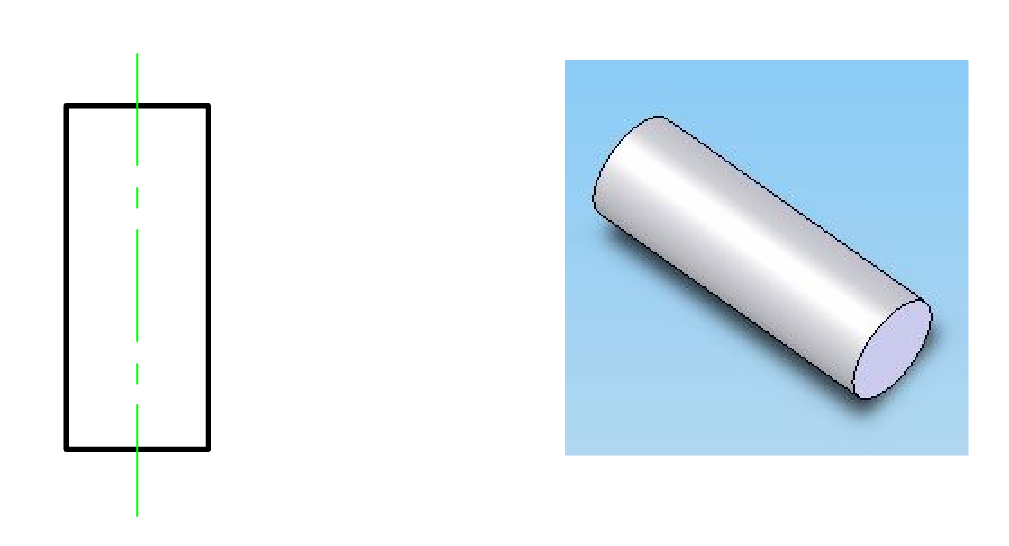
\includegraphics[width = 8 cm]{Images/ImagesDessinTechnique/axeRevolution.png}
    \caption{Utilisation de l'axe mixte dans la représentation d'un cylindre. Aucune autre vue n'est nécessaire.}
    \label{fig:my_label}
\end{figure}


\subsection{Représentation des arêtes}
Dans un plan, il faut représenter \textbf{toutes} les arêtes visibles dans cette vue.

\begin{figure}[H]
    \centering
    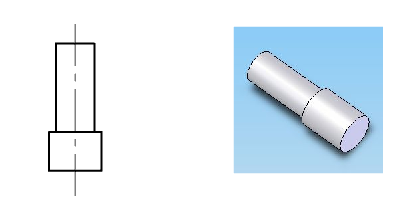
\includegraphics[width = 8cm]{Images/ImagesDessinTechnique/AretesCylindre.png}
    \caption{Représentation d'un cylindre à section variable. Il ne faut pas oublier l'arête faisant la délimitation entre les deux "parties"}
    \label{fig:my_label}
\end{figure}

Si l'on décide d'ajouter un plat au cylindre comme suit, on doit alors 
\begin{enumerate}
    \item Ajouter les nouvelles arêtes visibles sur le dessin
    \item Ajouter une seconde vue. En effet, l'unique vue précédente ne permet pas d'indiquer la "profondeur du plat".
\end{enumerate}

\begin{figure}[H]
    \centering
    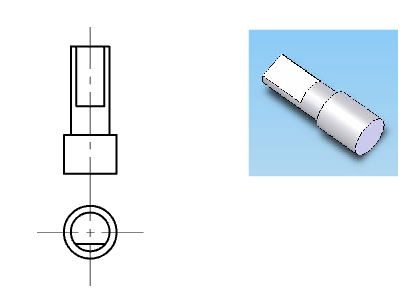
\includegraphics[width = 8cm]{Images/ImagesDessinTechnique/platCylindre.png}
    \caption{Ajout d'un plat au solide précédent}
    \label{fig:cylindrePlat}
\end{figure}



\subsection{Perçage de trous}

Si l'on souhaite percer un trou dans le plat du cylindre dessiné dans la figure \ref{fig:cylindrePlat}, il suffit d'ajouter sur la vue de face, un \textbf{cercle} ainsi que \textbf{son trait d'axe}.\\
Sans information supplémentaires, on considérera que le trou est traversant.\\

Il est également possible d'ajouter sur la vue du dessus la profondeur du trou. Cela doit se faire en trait discontinus car les arêtes sont cachées.

\begin{figure}[H]
    \centering
    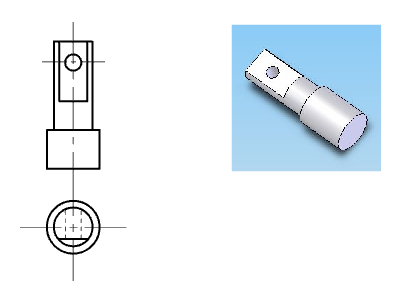
\includegraphics[width = 8cm]{Images/ImagesDessinTechnique/trouCylindre.png}
    \caption{Ajout d'un trou dans le solide.}
    \label{fig:my_label}
\end{figure}

Pour représenter un trou borgne, il faut alors rajouter les arêtes cachées dans la vue principale.\\
Un trou est percé avec un foret. Le bout d'un foret est pointu. Il ne faut donc pas oublier de rajouter la pointe dans le trous.

\begin{figure}[H]
    \centering
    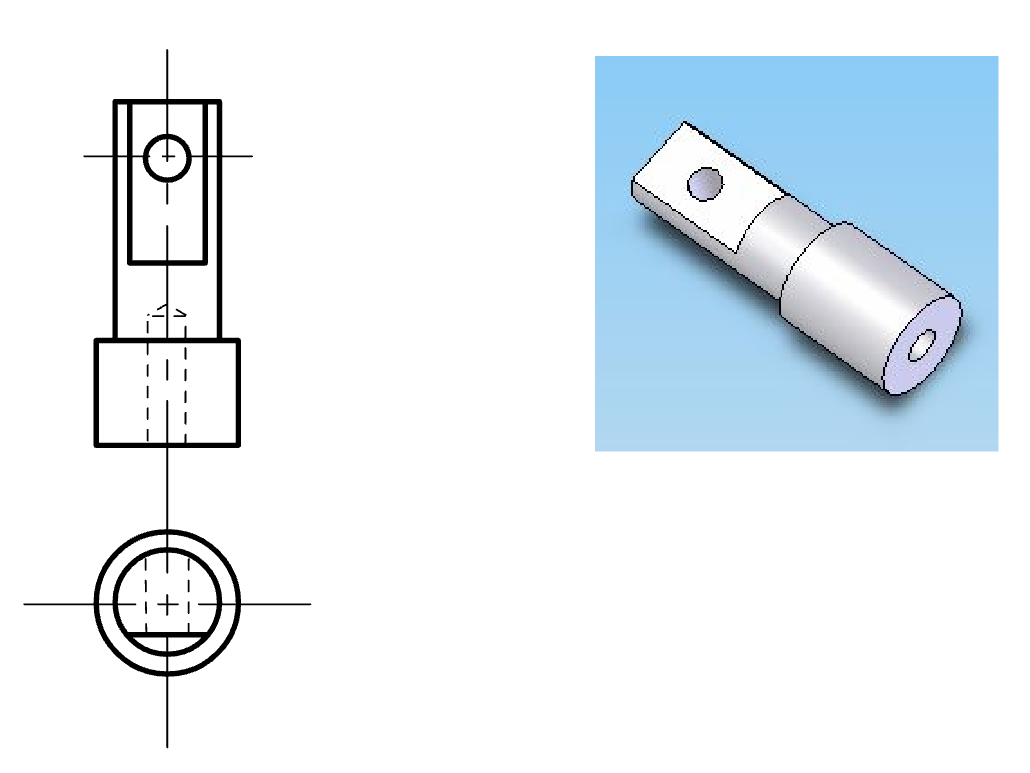
\includegraphics[width = 8cm]{Images/ImagesDessinTechnique/foretCyclindre.png}
    \caption{Perçage d'un trou borgne avec un foret}
    \label{fig:foret}
\end{figure}
